
%% bare_jrnl.tex
%% V1.4b
%% 2015/08/26
%% by Michael Shell
%% see http://www.michaelshell.org/
%% for current contact information.
%%
%% This is a skeleton file demonstrating the use of IEEEtran.cls
%% (requires IEEEtran.cls version 1.8b or later) with an IEEE
%% journal paper.
%%
%% Support sites:
%% http://www.michaelshell.org/tex/ieeetran/
%% http://www.ctan.org/pkg/ieeetran
%% and
%% http://www.ieee.org/

%%*************************************************************************
%% Legal Notice:
%% This code is offered as-is without any warranty either expressed or
%% implied; without even the implied warranty of MERCHANTABILITY or
%% FITNESS FOR A PARTICULAR PURPOSE!
%% User assumes all risk.
%% In no event shall the IEEE or any contributor to this code be liable for
%% any damages or losses, including, but not limited to, incidental,
%% consequential, or any other damages, resulting from the use or misuse
%% of any information contained here.
%%
%% All comments are the opinions of their respective authors and are not
%% necessarily endorsed by the IEEE.
%%
%% This work is distributed under the LaTeX Project Public License (LPPL)
%% ( http://www.latex-project.org/ ) version 1.3, and may be freely used,
%% distributed and modified. A copy of the LPPL, version 1.3, is included
%% in the base LaTeX documentation of all distributions of LaTeX released
%% 2003/12/01 or later.
%% Retain all contribution notices and credits.
%% ** Modified files should be clearly indicated as such, including  **
%% ** renaming them and changing author support contact information. **
%%*************************************************************************


% *** Authors should verify (and, if needed, correct) their LaTeX system  ***
% *** with the testflow diagnostic prior to trusting their LaTeX platform ***
% *** with production work. The IEEE's font choices and paper sizes can   ***
% *** trigger bugs that do not appear when using other class files.       ***                          ***
% The testflow support page is at:
% http://www.michaelshell.org/tex/testflow/



\documentclass[journal]{IEEEtran}
%
% If IEEEtran.cls has not been installed into the LaTeX system files,
% manually specify the path to it like:
% \documentclass[journal]{../sty/IEEEtran}





% Some very useful LaTeX packages include:
% (uncomment the ones you want to load)


% *** MISC UTILITY PACKAGES ***
%
%\usepackage{ifpdf}
% Heiko Oberdiek's ifpdf.sty is very useful if you need conditional
% compilation based on whether the output is pdf or dvi.
% usage:
% \ifpdf
%   % pdf code
% \else
%   % dvi code
% \fi
% The latest version of ifpdf.sty can be obtained from:
% http://www.ctan.org/pkg/ifpdf
% Also, note that IEEEtran.cls V1.7 and later provides a builtin
% \ifCLASSINFOpdf conditional that works the same way.
% When switching from latex to pdflatex and vice-versa, the compiler may
% have to be run twice to clear warning/error messages.






% *** CITATION PACKAGES ***
%
%\usepackage{cite}
% cite.sty was written by Donald Arseneau
% V1.6 and later of IEEEtran pre-defines the format of the cite.sty package
% \cite{} output to follow that of the IEEE. Loading the cite package will
% result in citation numbers being automatically sorted and properly
% "compressed/ranged". e.g., [1], [9], [2], [7], [5], [6] without using
% cite.sty will become [1], [2], [5]--[7], [9] using cite.sty. cite.sty's
% \cite will automatically add leading space, if needed. Use cite.sty's
% noadjust option (cite.sty V3.8 and later) if you want to turn this off
% such as if a citation ever needs to be enclosed in parenthesis.
% cite.sty is already installed on most LaTeX systems. Be sure and use
% version 5.0 (2009-03-20) and later if using hyperref.sty.
% The latest version can be obtained at:
% http://www.ctan.org/pkg/cite
% The documentation is contained in the cite.sty file itself.






% *** GRAPHICS RELATED PACKAGES ***
%
\ifCLASSINFOpdf
  % \usepackage[pdftex]{graphicx}
  % declare the path(s) where your graphic files are
  % \graphicspath{{../pdf/}{../jpeg/}}
  % and their extensions so you won't have to specify these with
  % every instance of \includegraphics
  % \DeclareGraphicsExtensions{.pdf,.jpeg,.png}
\else
  % or other class option (dvipsone, dvipdf, if not using dvips). graphicx
  % will default to the driver specified in the system graphics.cfg if no
  % driver is specified.
  % \usepackage[dvips]{graphicx}
  % declare the path(s) where your graphic files are
  % \graphicspath{{../eps/}}
  % and their extensions so you won't have to specify these with
  % every instance of \includegraphics
  % \DeclareGraphicsExtensions{.eps}
\fi
% graphicx was written by David Carlisle and Sebastian Rahtz. It is
% required if you want graphics, photos, etc. graphicx.sty is already
% installed on most LaTeX systems. The latest version and documentation
% can be obtained at:
% http://www.ctan.org/pkg/graphicx
% Another good source of documentation is "Using Imported Graphics in
% LaTeX2e" by Keith Reckdahl which can be found at:
% http://www.ctan.org/pkg/epslatex
%
% latex, and pdflatex in dvi mode, support graphics in encapsulated
% postscript (.eps) format. pdflatex in pdf mode supports graphics
% in .pdf, .jpeg, .png and .mps (metapost) formats. Users should ensure
% that all non-photo figures use a vector format (.eps, .pdf, .mps) and
% not a bitmapped formats (.jpeg, .png). The IEEE frowns on bitmapped formats
% which can result in "jaggedy"/blurry rendering of lines and letters as
% well as large increases in file sizes.
%
% You can find documentation about the pdfTeX application at:
% http://www.tug.org/applications/pdftex





% *** MATH PACKAGES ***
%
%\usepackage{amsmath}
% A popular package from the American Mathematical Society that provides
% many useful and powerful commands for dealing with mathematics.
%
% Note that the amsmath package sets \interdisplaylinepenalty to 10000
% thus preventing page breaks from occurring within multiline equations. Use:
%\interdisplaylinepenalty=2500
% after loading amsmath to restore such page breaks as IEEEtran.cls normally
% does. amsmath.sty is already installed on most LaTeX systems. The latest
% version and documentation can be obtained at:
% http://www.ctan.org/pkg/amsmath





% *** SPECIALIZED LIST PACKAGES ***
%
%\usepackage{algorithmic}
% algorithmic.sty was written by Peter Williams and Rogerio Brito.
% This package provides an algorithmic environment fo describing algorithms.
% You can use the algorithmic environment in-text or within a figure
% environment to provide for a floating algorithm. Do NOT use the algorithm
% floating environment provided by algorithm.sty (by the same authors) or
% algorithm2e.sty (by Christophe Fiorio) as the IEEE does not use dedicated
% algorithm float types and packages that provide these will not provide
% correct IEEE style captions. The latest version and documentation of
% algorithmic.sty can be obtained at:
% http://www.ctan.org/pkg/algorithms
% Also of interest may be the (relatively newer and more customizable)
% algorithmicx.sty package by Szasz Janos:
% http://www.ctan.org/pkg/algorithmicx




% *** ALIGNMENT PACKAGES ***
%
%\usepackage{array}
% Frank Mittelbach's and David Carlisle's array.sty patches and improves
% the standard LaTeX2e array and tabular environments to provide better
% appearance and additional user controls. As the default LaTeX2e table
% generation code is lacking to the point of almost being broken with
% respect to the quality of the end results, all users are strongly
% advised to use an enhanced (at the very least that provided by array.sty)
% set of table tools. array.sty is already installed on most systems. The
% latest version and documentation can be obtained at:
% http://www.ctan.org/pkg/array


% IEEEtran contains the IEEEeqnarray family of commands that can be used to
% generate multiline equations as well as matrices, tables, etc., of high
% quality.




% *** SUBFIGURE PACKAGES ***
%\ifCLASSOPTIONcompsoc
%  \usepackage[caption=false,font=normalsize,labelfont=sf,textfont=sf]{subfig}
%\else
%  \usepackage[caption=false,font=footnotesize]{subfig}
%\fi
% subfig.sty, written by Steven Douglas Cochran, is the modern replacement
% for subfigure.sty, the latter of which is no longer maintained and is
% incompatible with some LaTeX packages including fixltx2e. However,
% subfig.sty requires and automatically loads Axel Sommerfeldt's caption.sty
% which will override IEEEtran.cls' handling of captions and this will result
% in non-IEEE style figure/table captions. To prevent this problem, be sure
% and invoke subfig.sty's "caption=false" package option (available since
% subfig.sty version 1.3, 2005/06/28) as this is will preserve IEEEtran.cls
% handling of captions.
% Note that the Computer Society format requires a larger sans serif font
% than the serif footnote size font used in traditional IEEE formatting
% and thus the need to invoke different subfig.sty package options depending
% on whether compsoc mode has been enabled.
%
% The latest version and documentation of subfig.sty can be obtained at:
% http://www.ctan.org/pkg/subfig




% *** FLOAT PACKAGES ***
%
%\usepackage{fixltx2e}
% fixltx2e, the successor to the earlier fix2col.sty, was written by
% Frank Mittelbach and David Carlisle. This package corrects a few problems
% in the LaTeX2e kernel, the most notable of which is that in current
% LaTeX2e releases, the ordering of single and double column floats is not
% guaranteed to be preserved. Thus, an unpatched LaTeX2e can allow a
% single column figure to be placed prior to an earlier double column
% figure.
% Be aware that LaTeX2e kernels dated 2015 and later have fixltx2e.sty's
% corrections already built into the system in which case a warning will
% be issued if an attempt is made to load fixltx2e.sty as it is no longer
% needed.
% The latest version and documentation can be found at:
% http://www.ctan.org/pkg/fixltx2e


%\usepackage{stfloats}
% stfloats.sty was written by Sigitas Tolusis. This package gives LaTeX2e
% the ability to do double column floats at the bottom of the page as well
% as the top. (e.g., "\begin{figure*}[!b]" is not normally possible in
% LaTeX2e). It also provides a command:
%\fnbelowfloat
% to enable the placement of footnotes below bottom floats (the standard
% LaTeX2e kernel puts them above bottom floats). This is an invasive package
% which rewrites many portions of the LaTeX2e float routines. It may not work
% with other packages that modify the LaTeX2e float routines. The latest
% version and documentation can be obtained at:
% http://www.ctan.org/pkg/stfloats
% Do not use the stfloats baselinefloat ability as the IEEE does not allow
% \baselineskip to stretch. Authors submitting work to the IEEE should note
% that the IEEE rarely uses double column equations and that authors should try
% to avoid such use. Do not be tempted to use the cuted.sty or midfloat.sty
% packages (also by Sigitas Tolusis) as the IEEE does not format its papers in
% such ways.
% Do not attempt to use stfloats with fixltx2e as they are incompatible.
% Instead, use Morten Hogholm'a dblfloatfix which combines the features
% of both fixltx2e and stfloats:
%
% \usepackage{dblfloatfix}
% The latest version can be found at:
% http://www.ctan.org/pkg/dblfloatfix




%\ifCLASSOPTIONcaptionsoff
%  \usepackage[nomarkers]{endfloat}
% \let\MYoriglatexcaption\caption
% \renewcommand{\caption}[2][\relax]{\MYoriglatexcaption[#2]{#2}}
%\fi
% endfloat.sty was written by James Darrell McCauley, Jeff Goldberg and
% Axel Sommerfeldt. This package may be useful when used in conjunction with
% IEEEtran.cls'  captionsoff option. Some IEEE journals/societies require that
% submissions have lists of figures/tables at the end of the paper and that
% figures/tables without any captions are placed on a page by themselves at
% the end of the document. If needed, the draftcls IEEEtran class option or
% \CLASSINPUTbaselinestretch interface can be used to increase the line
% spacing as well. Be sure and use the nomarkers option of endfloat to
% prevent endfloat from "marking" where the figures would have been placed
% in the text. The two hack lines of code above are a slight modification of
% that suggested by in the endfloat docs (section 8.4.1) to ensure that
% the full captions always appear in the list of figures/tables - even if
% the user used the short optional argument of \caption[]{}.
% IEEE papers do not typically make use of \caption[]'s optional argument,
% so this should not be an issue. A similar trick can be used to disable
% captions of packages such as subfig.sty that lack options to turn off
% the subcaptions:
% For subfig.sty:
% \let\MYorigsubfloat\subfloat
% \renewcommand{\subfloat}[2][\relax]{\MYorigsubfloat[]{#2}}
% However, the above trick will not work if both optional arguments of
% the \subfloat command are used. Furthermore, there needs to be a
% description of each subfigure *somewhere* and endfloat does not add
% subfigure captions to its list of figures. Thus, the best approach is to
% avoid the use of subfigure captions (many IEEE journals avoid them anyway)
% and instead reference/explain all the subfigures within the main caption.
% The latest version of endfloat.sty and its documentation can obtained at:
% http://www.ctan.org/pkg/endfloat
%
% The IEEEtran \ifCLASSOPTIONcaptionsoff conditional can also be used
% later in the document, say, to conditionally put the References on a
% page by themselves.




% *** PDF, URL AND HYPERLINK PACKAGES ***
%
%\usepackage{url}
% url.sty was written by Donald Arseneau. It provides better support for
% handling and breaking URLs. url.sty is already installed on most LaTeX
% systems. The latest version and documentation can be obtained at:
% http://www.ctan.org/pkg/url
% Basically, \url{my_url_here}.




% *** Do not adjust lengths that control margins, column widths, etc. ***
% *** Do not use packages that alter fonts (such as pslatex).         ***
% There should be no need to do such things with IEEEtran.cls V1.6 and later.
% (Unless specifically asked to do so by the journal or conference you plan
% to submit to, of course. )

\usepackage{xcolor}
\usepackage[utf8]{inputenc}
\usepackage[pdftex]{graphicx}
\graphicspath{{Figures/}}
\DeclareGraphicsExtensions{.pdf,.jpeg,.png}
\usepackage{cite}
%\usepackage{url}
\usepackage{textcomp}
\usepackage{color}
\usepackage[colorlinks]{hyperref}



% correct bad hyphenation here
\hyphenation{op-tical net-works semi-conduc-tor Fire-Kernel}


\begin{document}
%
% paper title
% Titles are generally capitalized except for words such as a, an, and, as,
% at, but, by, for, in, nor, of, on, or, the, to and up, which are usually
% not capitalized unless they are the first or last word of the title.
% Linebreaks \\ can be used within to get better formatting as desired.
% Do not put math or special symbols in the title.

\title{Topic: Security of In-vehicle Communication}
%
%
% author names and IEEE memberships
% note positions of commas and nonbreaking spaces ( ~ ) LaTeX will not break
% a structure at a ~ so this keeps an author's name from being broken across
% two lines.
% use \thanks{} to gain access to the first footnote area
% a separate \thanks must be used for each paragraph as LaTeX2e's \thanks
% was not built to handle multiple paragraphs
%

\author{

\IEEEauthorblockN{Julian Pfeifer}

}




% note the % following the last \IEEEmembership and also \thanks -
% these prevent an unwanted space from occurring between the last author name
% and the end of the author line. i.e., if you had this:
%
% \author{....lastname \thanks{...} \thanks{...} }
%                     ^------------^------------^----Do not want these spaces!
%
% a space would be appended to the last name and could cause every name on that
% line to be shifted left slightly. This is one of those "LaTeX things". For
% instance, "\textbf{A} \textbf{B}" will typeset as "A B" not "AB". To get
% "AB" then you have to do: "\textbf{A}\textbf{B}"
% \thanks is no different in this regard, so shield the last } of each \thanks
% that ends a line with a % and do not let a space in before the next \thanks.
% Spaces after \IEEEmembership other than the last one are OK (and needed) as
% you are supposed to have spaces between the names. For what it is worth,
% this is a minor point as most people would not even notice if the said evil
% space somehow managed to creep in.




% The only time the second header will appear is for the odd numbered pages
% after the title page when using the twoside option.
%
% *** Note that you probably will NOT want to include the author's ***
% *** name in the headers of peer review papers.                   ***
% You can use \ifCLASSOPTIONpeerreview for conditional compilation here if
% you desire.




% If you want to put a publisher's ID mark on the page you can do it like
% this:
%\IEEEpubid{0000--0000/00\$00.00~\copyright~2015 IEEE}
% Remember, if you use this you must call \IEEEpubidadjcol in the second
% column for its text to clear the IEEEpubid mark.



% use for special paper notices
%\IEEEspecialpapernotice{(Invited Paper)}




% make the title area
\maketitle

% As a general rule, do not put math, special symbols or citations
% in the abstract or keywords.
\begin{abstract}
% !TEX root = ../report.tex

While IoT devices get more and more widely used, embedded boards are already a
central part of every car for several years now. Sensors and embedded boards for
car control are connected via a multitude of networks. The most widely used of
these networks, the Controller Area Network (CAN), was designed in the eighties
with no security in mind because these networks were closed off. But nowadays
vehicles have a multitude of interfaces to outside networks, so there is a dire
need to modernise the in-vehicle networks with appropriate security measures....tbd

\end{abstract}

% Note that keywords are not normally used for peerreview papers.
%\begin{IEEEkeywords}
%IoT, Operating System, Internet of Things
%\end{IEEEkeywords}






% For peer review papers, you can put extra information on the cover
% page as needed:
% \ifCLASSOPTIONpeerreview
% \begin{center} \bfseries EDICS Category: 3-BBND \end{center}
% \fi
%
% For peerreview papers, this IEEEtran command inserts a page break and
% creates the second title. It will be ignored for other modes.
\IEEEpeerreviewmaketitle


% !TEX root = ../report.tex

\section{Introduction}

The Internet of things (IoT) is a continuously growing network of commonplace
devices. They can be physical like wireless sensors and smart phones or virtual
like services. The IoT transforms how we interact with our environment. Today
almost any electronic device can be bought as a smart version like microwaves,
washing machines, light bulbs, door locks and many other "things". All these
belong to the IoT network. The IoT has several application domains. It can be
used personally or in enterprises \cite{Mahmoud2015}. The personal and social
application domain is for connecting people to their environment and to other
people. The industries and enterprises domain enables different activities in
and between organizations of for example the finance and banking sector. Also
IoT can be used in for example breeding or energy management where it is used
for service and utility monitoring. The last application domain is
transportation. Which encompasses smart cars and infrastructure like traffic
lights.

Ever since there were the first electronic systems to assist drivers in control
of their cars there were Electronic Control Units (ECUs) included in these
vehicles. ECUs consist of micro-controllers and sensors. Nowadays cars have not
only normal Driver Assistance Systems like antilock breaking systems. They also
have Advanced Driver Assistance Systems (ADAS) which help people with
safety-critical functionality like parking or emergency breaking. To realize all
these functions a multitude of in-vehicle networks (IVNs) is needed to connect
all the ECUs and the sensors. These IVNs were originally closed off and had no
connection to other networks. So they were designed with no security in mind
whatsoever. Recently, cars have been connected to a multitude of networks like
3G/4G mobile phone networks, Bluetooth and vehicular ad hoc networks (IEEE
802.11p). So the IVNs have become vulnerable to different types of attacks while
joining the IoT. The most used type of IVN today is still the Controller Area
Network (CAN). It was introduced in 1983 by the Robert Bosh GmbH. Because in
these days IVNs were closed of there were no security features included in the
CAN protocol like encryption or message authentication \cite{Avatefipour2017}.
This absence of inherent security features in the protocol led to successful
demonstrations of security breaches \cite{Koscher2010}. It was possible to
reprogram ECUs via physical and wireless connections. The car could even be
monitored and controlled remotely. Since then there have been many automotive
attack demonstrations \cite{Hoppe2011,Checkoway2011,Cheah2017}.

This report focuses on recent CAN authentication research. Two initially
proposed authentication protocols named LeiA and vatiCAN secure the CAN network
against adversaries that do not control code execution on ECUs in the network
\cite{Nurnberger2016,Radu2016}. Later these protocols were improved by VulCAN
which is an efficient approach to implement secure distributed automotive
control software on lightweight trusted computing platforms \cite{VanBulck2017}.
VulCAN adds another layer of security by relying on trusted hardware and a
minimal software Trusted Computing Base (TCB). Additionally it was shown that
VulCAN provides sufficient performance to be used in automotive real-time
applications.

In the following chapter \ref{sec:communication-networks} I will provide an
overview of different IVNs like CAN, Time-Triggered Networks, Low-Cost
Automotive Networks and more. Also I will introduce the general types of
security measures in IVNs. Afterwards chapters \ref{sec:leia} and
\ref{sec:vatican} will explain LeiA and vatiCAN and how each of them work in
general. Chapter \ref{sec:vulcan} will talk in depth about VulCAN. I will
explain how it achieves improvements over LeiA and vatiCAN using Sancus 2.0.
Finally there will be a discussion in chapter \ref{sec:discussion} connecting security in IVNs to security in
the general IoT sector and the world wide web.

% !TEX root = ../report.tex


\section{In-vehicle Communication Networks and Security}
\label{sec:communication-networks}

CAN Network, Time-Triggered Networks, Low-Cost Automotive Networks, Multimedia
and Infotainment Networks, Automotive Ethernet \cite{Navet2017}

Security Measures: Controller Authentication, Encrypted Communication, Gateway
Firewalls \cite{Lemke2006}


\section{LeiA: Lightweight Authentication Protocol for CAN}

Overview of LeiA \cite{Radu2016}


\section{VatiCAN: Vetted, authenticated CAN bus}

Overview of vatiCAN \cite{Nurnberger2016}

% \begin{figure}[h]
% 	\centering
% 	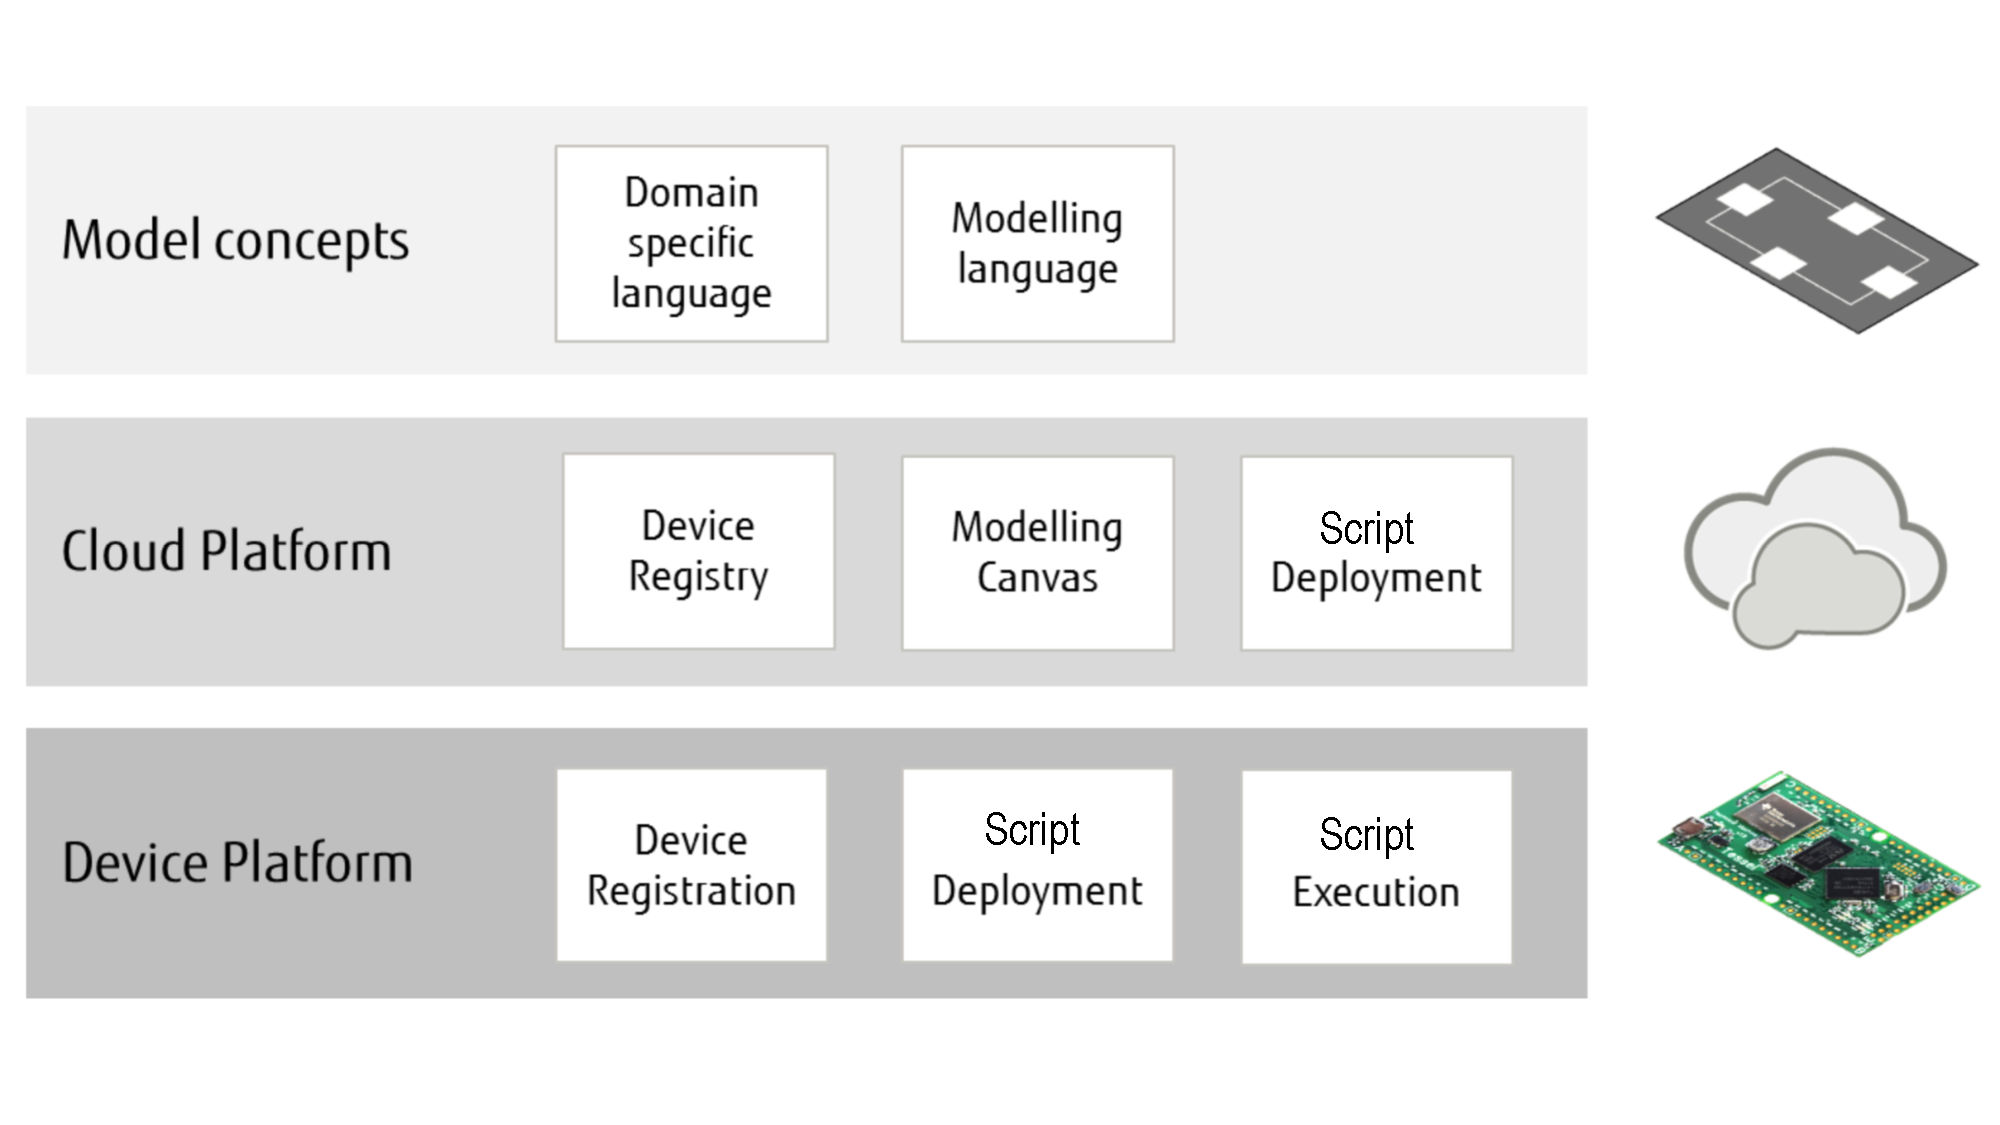
\includegraphics[width=0.8\linewidth]{Figures/sample-figure}
% 	\caption[]{Sample figure.}
% 	\label{fig:sample-figure}
% \end{figure}

% !TEX root = ../report.tex



\section{LeiA:\ Lightweight Authentication Protocol for CAN}\label{sec:leia}

The LeiA~\cite{Radu2016} protocol was created to authenticate messages in IVNs
to prevent attackers from imposing as participants. The authors of LeiA assume
that an attacker got access to the network but did not compromise the target
ECU\@. So the attacker is possible to read CAN traffic and send out messages. It
uses an unidirectional authentication using symmetric keys. Every participant in
the network using the LeiA authentication needs to store information per
relevant CAN identifier it wants to send or receive information on:

\begin{itemize}
    \item CAN identifier
    \item A long term 128-bit symmetric key used in generating the corresponding
    session key.
    \item The epoch is a 56-bit counter which is increased every time the
    network is restarted or the message counter overflows. It is used in the
    generation of the session key.
    \item A 16-bit message counter included in the data frame. It is used for
    MAC generation.
    \item A 128-bit session key used for generating the MAC\@. It is regenerated
    when the epoch changes to limit the number of messages authenticated per
    session key.
\end{itemize}

The authors of LeiA assume that the symmetric keys and identifiers are stored in
tamper-resistant memory. So it should require physical access to the vehicle to
update these keys.

The session key generation is done at the start to initialize the system. So for
every CAN identifier id such a session key is generated by the following steps:

\begin{enumerate}
    \item increment current epoch value for identifier id by one
    \item generate the session key by providing the epoch and symmetric key to
    the MAC generation algorithm.
    \item reset the message counter to zero.
\end{enumerate}

\begin{figure}[ht]
    \centering
    \captionsetup{justification=centering}
	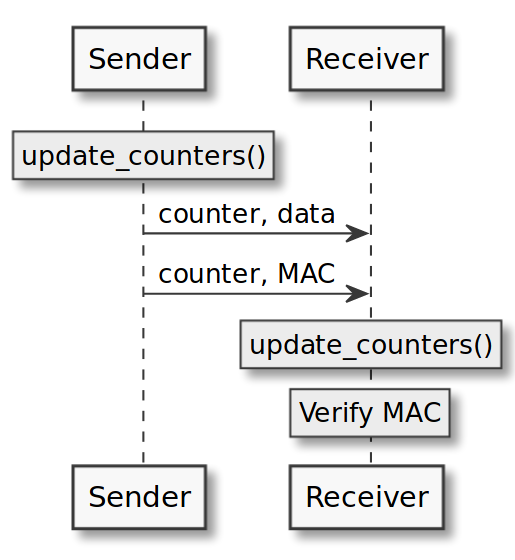
\includegraphics[width=0.6\linewidth]{Figures/LeiA_sending_msg.png}
	\caption[]{Sending an authenticated Message using LeiA}\label{fig:leia_sending_msg}
\end{figure}

Before sending an authenticated message with LeiA, first the message counter has
to be increased. Then the data and the MAC are sent over the corresponding CAN
identifier. The receivers will increase its own message counter for the
identifier and then verify the received MAC for the data. If this authentication
is successful the data is processed (see Fig.~\ref{fig:leia_sending_msg}).

\begin{figure}[ht]
    \centering
    \captionsetup{justification=centering}
	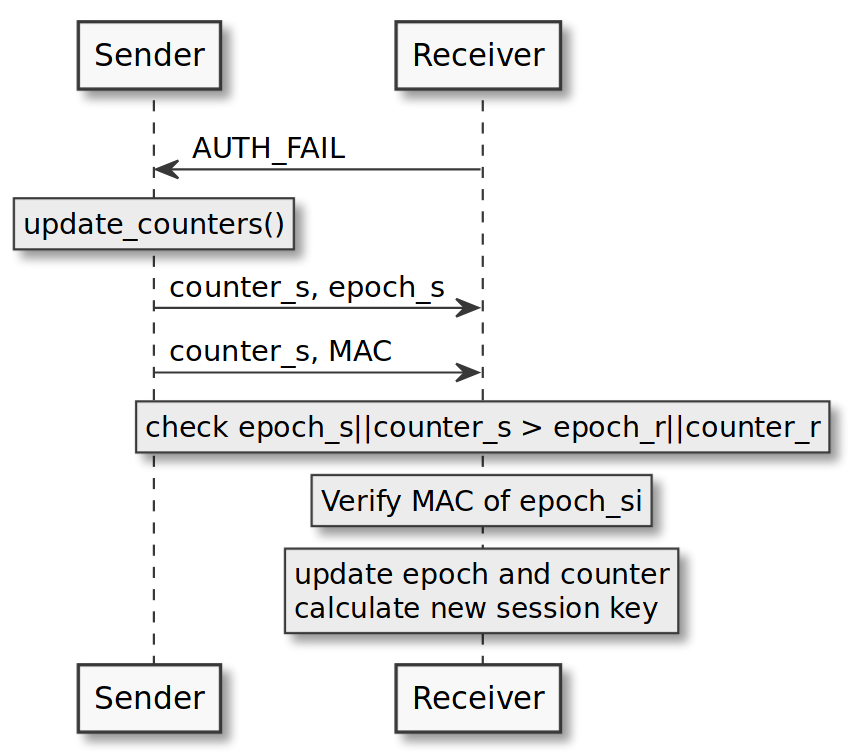
\includegraphics[width=1\linewidth]{Figures/LeiA_resync.png}
    \caption[]{Message resynchronisation after a failed message authentication 
    between Sender s and Receiver r using LeiA.}\label{fig:leia_resync}
\end{figure}

If the authentication of a message fails a resynchronization between sender and
receiver is needed (see Fig.~\ref{fig:leia_resync}). This means they do not use
the same session key because the epoch is out of sync. In this case the receiver
will send an AUTH\_FAIL message to signal the desynchronization to the original
sender of the message that is causing the authentication problem. The sender
will then send out its current epoch value and a corresponding MAC generated
from the epoch. The receiver will accept this new epoch and counter value from
the sender if:

\begin{enumerate}
    \item The concatenated value of the received epoch and counter are higher
    than its own (\( epoch_{rec} || counter_{rec}~>~epoch_{own} || counter_{own}
    \)). This check prevents replay attacks with older messages. 
    \item The provided MAC for the new epoch is successfully verified with a new
    generated session key fitting this epoch.
\end{enumerate}

Only if both conditions hold, the new received value for epoch and counter are
used to update the values of the out of sync receiver. After this the sender
will resume normal sending of messages. 

In general there is a setup/initiation phase at the start. In this phase the
epoch counter will be increased and the message counter will be reset to zero.
Additionally the session keys will be generated from the long term symmetric
keys and the corresponding epoch value. After the initiation the sending of
messages can begin. Before each message the sender will update its message
counter. The receiver will update its own counter independently and then verify
the provided MAC\@. If there occurs an authentication error the resynchronization
procedure will be triggered. The complete outline of the protocol is given in
Figure~\ref{fig:leia_outline}.

\begin{figure}[ht]
    \centering
    \captionsetup{justification=centering}
	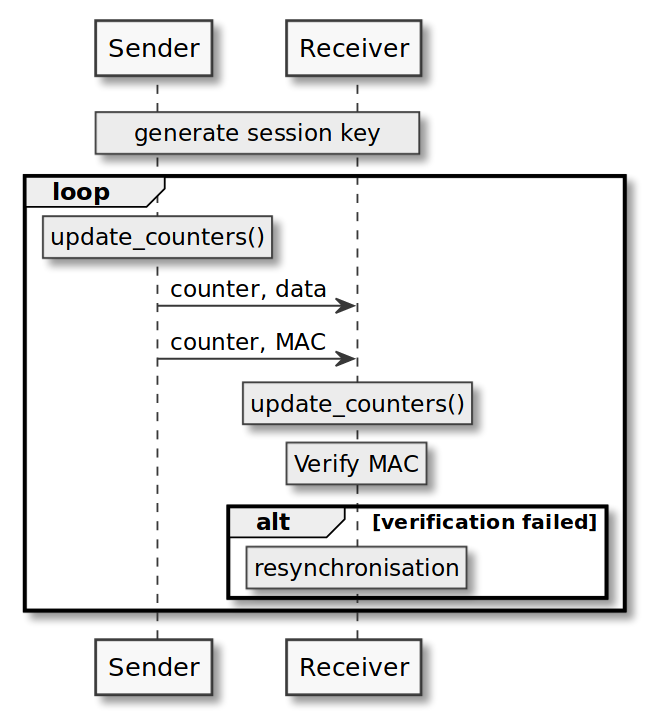
\includegraphics[width=0.9\linewidth]{Figures/LeiA_outline.png}
	\caption[]{LeiA protocol outline.}\label{fig:leia_outline}
\end{figure}

To be able to use an authentication protocol in the in-vehicle network
environment it needs to be lightweight. It can not introduce considerable
latency or even contain too much code because the ECUs have very limited
processing and memory capabilities. Therefor LeiA uses the MAC algorithm also for
generating the session keys so the code can be reused at that point. The session
keys are used for compensation of the moderate security provided by the
lightweight cryptography. So only a maximum of \( 2^{16} \) messages are secured
by the same session key. After that the epoch has to change and a new session
key is used to generate the MACs. In case of a restart of the system the epoch
and thus the session key will change too. This restricts the use of a
compromised session key.

The LeiA protocol includes the counter in the extended identifier field of the
CAN message which is normally used to extend the range of possible identifiers.
The first two bits of this field are used to signal which kind of data is
included in the payload field: data, MAC of data, epoch or MAC of an epoch.
Every ECU using the LeiA protocol needs three communication channels. Therefor
it needs three different identifiers. There is a data channel, an authentication
channel and an authentication error channel. As seen in
Figure~\ref{fig:leia_sending_msg}, every time data is sent there are two
messages sent out. One with the data and one with the MAC for the data. The data
is sent over the data channel and the MAC is sent over the authentication
channel. The AUTH\_FAIL messages (see Figure~\ref{fig:leia_resync}) are sent
over the authentication error channel. So every ECU broadcasting messages in the
network need to subscribe to all authentication error channels from its
subscribers.

If the LeiA protocol is used like that the messages sent roughly double because
for every data message a message with a corresponding MAC is sent out. However
not all ECUs need the same level of security. So LeiA provides a scaling
mechanism by not sending out a MAC for every data message. It
is customizable for every ECU after how many messages a MAC is sent out. If there is a low
security component there could be only an authentication message sent out for
every tenth message.

In~\cite{Radu2016} the authors show that the LeiA protocol is secure against
probabilistic polynomial time adversaries that can freely interact with protocol
participants meaning they have only a negligible chance of successfully
deceiving one of the participants to have another valid identity. The protocol
provides no security against fully compromised ECUs. These possess all the keys
they use to broadcast and listen with normally. So a compromised node can listen
and broadcast on all these channels and create valid MACs for them. This is an
inherent problem of the used symmetric key cryptography. LeiA provides no
security against denial of service (DoS) attacks. But it helps by not parsing
data from messages with failed authentications.

\section{vatiCAN:\ vetted, authenticated CAN bus}\label{sec:vatiCAN}

The vetted, authenticated CAN bus protocol (vatiCAN)~\cite{Nurnberger2016} was
designed to provide maximum security while providing full backwards
compatibility to standard CAN\@. vatiCAN provides two core functionalities. The
most important functionality is of course the authentication of messages and
senders. Secondly, the protocol provides spoof detection for ECUs to detect
spoofed messages with their own identifier. Additionally the vatiCAN protocol
provides protection against replay attacks. Moreover it defines a changed CAN
arbitration to provide spoof prevention.

The authors of vatiCAN define six challenges that a CAN authentication protocol
needs to face:

\begin{enumerate}
    \item[C1] Since CAN has hard real time constraints, security mechanisms for
    it can only add acceptable communication overhead not causing to
    significantly increase latency and message collisions. 
    \item[C2] Heavy-duty crypto can not be used since ECUs have very limited
    computational power and memory available.
    \item[C3] CAN messages have only a maximum payload of 8 bytes. Either the
    messages fit into these 64-bit or the data is broken up into multiple
    messages.
    \item[C4] Every vehicle must have its own cryptographic keys to not be able
    to extract working keys from another vehicle.
    \item[C5] Non-critical ECUs should not be modified to be able to keep on
    using existing hardware. So compatibility is needed with the standard CAN
    protocol.
    \item[C6] Authenticated CAN messages need to be protected against replay
    attacks without introducing a global state since CAN is a stateless
    protocol.
\end{enumerate}

vatiCAN's authors assume that an attacker does not have physical access to the
vehicle but compromised an ECU wirelessly. Furthermore they assume that the
attacker did not compromise the real target ECU\@. vatiCAN provides no security
against compromised ECUs sending authenticated messages with their own
identifiers. So the attacker needs to impersonate another ECU with the help of
the compromised one. She is also capable of reading all of the CAN messages and
learn about the other ECUs identities.

The message organization in vatiCAN uses separate messages for the
authentication. The payload of the original data message is not modified in any
way. For the authentication message the next identifier with lower priority is
used (id plus one). This assures that both, the data and the authentication
message have effectively the same priority with the authentication message
not effecting the data message. This design was chosen with challenges C1 and C5
in mind. The receipt of data messages is not influenced by the protocol and
unmodified ECUs can still read the data messages without any changes.

For message authentication (concerning C2 and C3) a lightweight key-hashed
message authentication code (HMAC) has been chosen. In particular the Keccak
algorithm standardized as SHA-3 has been used since it was shown to be the
fastest hash function on Atmel embedded microcontrollers~\cite{Eisenbarth2012}.
An input to the hash function of 128~bit size is chosen containing the 64~bit
data payload plus the identifier for the corresponding data message and a nonce
(explained below). So this HMAC is the payload of the authentication message
which is sent additionally to the data message as described above.

The symmetric keys used in the hashing function is chosen to be of 128~bit
length and injected into the ECUs during assembly (C4). This leads to key
updates of multiple ECUs when an ECU is replaced. Gladly ECUs can normally be
upgraded through the on-board diagnostics port. So this is no problem and is
preferable to a dynamic key-agreement procedure like a Diffie-Hellman key
exchange because these are non-trivial to implement on an embedded
microcontroller.

To prevent replay attacks (C6) of any kind a nonce is used. These nonce values
need to result in different values of HMACs when used in their generation. For
every identifier a counter is used as the nonce which is incremented after every
message sent. The receiver of an HMAC needs to know the counter value to verify
the authenticity. Since the sender and its receivers can get out of sync due to
lost messages a synchronization mechanism is needed. This is accomplished by a
global Nonce Generator. It periodically sends out new values which all ECUs then
use as the next counter value for their identifier after using the current
value. So the nonce/counter values are no secret and the attacker can know
them without problem. However without the secret symmetric keys for each
identifier the nonce is useless because no valid HMACs can be computed without
these keys. When two nodes get out of sync in regard to the nonce there is a
``deaf'' time where no message can be authenticated by the receiver until the
next global nonce value is published by the Nonce Generator. See
Figure~\ref{fig:vatiCAN_deaf_time} for an overview. The authors of vatiCAN
propose an interval of 50~milliseconds for sending out global nonce values. This
would be 1\% of the bandwidth of a 500~kBit/s CAN network.

\begin{figure}[ht]
    \centering
    \captionsetup{justification=centering}
	\includegraphics[width=0.8\linewidth]{Figures/vatiCAN_deaf_time.png}
	\caption[]{Nonce Generator sending out new nonce value}\label{fig:vatiCAN_deaf_time}
\end{figure}

Due to the data message arriving before the authentication message, the receiver
can start calculating the HMAC of the received payload. So the sender and
receiver can calculate the HMAC in parallel and when the HMAC calculated by the
sender is received, the receiver can directly compare the HMAC with its own
calculation (See Fig.~\ref{fig:vatiCAN_sending_msg})

\begin{figure}[ht]
    \centering
    \captionsetup{justification=centering}
	\includegraphics[width=0.8\linewidth]{Figures/vatiCAN_sending_msg.png}
	\caption[]{Sending an authenticated Message using vatiCAN}\label{fig:vatiCAN_sending_msg}
\end{figure}

An ECU is easily able to identify spoofed messages of its own identifier under
the prerequisite that every ECU has its own identifier. They can simply look out
for received messages with their own identifier. If then the CRC checksum is
destroyed with dominant bits while it is sent the whole spoofed message will be
dropped by every recipient. Sadly it is not possible to destroy the CRC checksum
without modifying the CAN transceiver chip since the CRC is normally handled by
the hardware. The authors propose to use such a modified transceiver chip for
their added ECU the Nonce Generator because this component has to be added newly
anyway for vatiCAN to work. So no attacker will be possible to impersonate the
Nonce Generator and control the nonce values of the other ECUs.

The authors of vatiCAN made a Hardware-in-the-Loop-Test with an instrument
cluster, accelerator and brake pedals, ATmega microcontrollers and CAN bus
controller chips on top of a bench~\cite{Nurnberger2016}. They implemented
vatiCAN as a library for the Arduino development environment for Atmel's AVR
microcontrollers. They made a performance evaluation of their protocol and found
out that receiving an authenticated message takes 3.3~ms longer than receiving a
message without vatiCAN authentication. It was measured on an ATmega 8~bit
microcontroller which is the low end of performance for embedded boards in
vehicles. The 3.3~ms are not to be underrated. They have an impact of 0.09~m
while driving with 100~km/h on a highway.

Van Bulck et al.\ show in~\cite{VanBulck2017} that an advanced replay attack
based on the generalized birthday problem (probability theory) is possible
against the vatiCAN protocol. This is possible due to the frequent random nonce
generation. After recording only 30 minutes of traffic it is possible to start
replaying authenticated messages.


\section{VulCAN:\ Vehicular Component Authentication and Software Isolation}\label{sec:vulcan}

VulCAN~\cite{VanBulck2017} is in essence no fully defined protocol but defines
only the main aspects of one that is largely compatible with every
AUTOSAR-compliant protocol. VulCAN extends such a compatible protocol if it is
implemented with the VulCAN approach by several system-level security
guarantees. The authors call this to ``vulcanize'' a protocol.

\subsection{Sancus}\label{subsec:sancus}

To achieve this, VulCAN is built on top of Sancus~2.0~\cite{Noorman}. Sancus is
a protected module architecture (PMA) that extends the embedded OpenMSP430
processor. It provides a hardware-only TCB extending the memory access logic and
processor instruction set. Sancus uses a hardware-level program counter-based
access control mechanism which secures the private data section of a software
component. So only the responsible code section can access its corresponding
private data section. Additionally this code section can only be entered through
one specific entry point. With this functionalities it is possible to run
multiple mutually distrusting software components in the same address space
without being able to spy on each others secrets. It is also possible to build
secured driver protected modules (PMs). They can hold exclusive access to
Memory-Mapped I/O devices. These driver PMs need to be written in assembly using
only registers to store data because Sancus only provides one contiguous private
data section. 

Sancus extends the processor with a cryptographic core. This enables
hardware-level authenticated encryption, key derivation and key storage
functionality. To enable remote / local attestation and secured communication
Sancus employs a three level key hierarchy. The root level of this hierarchy
consists of a hardware-level node master key. There exists exactly one of these
for each embedded computing node that is only known to the owner of this node.
Each independent vendor that installs software on this node is assigned a vendor
identity. From vendor identity and master key a vendor key can be calculated.
These vendor keys build the second level of the hierarchy. Lastly, the third
level of the hierarchy consists of module keys for each PM running on the
embedded node. The module keys are calculated from the vendor keys plus the
corresponding module identity. This module identity contains all content from
the code section plus the load addresses of both memory sections of the PM\@.
Upon finishing to load a PM the Sancus-enabled processor will compute the module
key and store it in a hardware-level secured memory area. The computed module
key can only be used by the respective PM\@. Independent from this calculation
the vendor who possesses also the vendor key and module identity can calculate
the module key. So it is easy to check the integrity of the PM with a simple
challenge by the vendor using the module key. If the loaded module was modified
in any way the module key will not match. This results in the ability to create
a secured communication either using the module key or another in-memory key.
The module keys calculated by the Sancus hardware also make it possible to
distrust the system software running on the embedded nodes. This reduces the TCB
to the PMs running on the node which makes formal verifications much easier.
Additionally the cryptography core provides hardware primitives for efficient
cryptographic calculations which can be used by the PMs. Furthermore Sancus
provides secure linking between two PMs on the same embedded node and comes with
a modified C compiler automating PM creation and hiding low-level concerns.

\subsection{Vulcanized CAN components}

The software-only protocols LeiA~\cite{Radu2016} and
vatiCAN~\cite{Nurnberger2016} described in the two chapters above are very
similar. They use pre-shared symmetric keys between sender and receiver.
Additionally both use a monotonically increasing nonce protecting against replay
attacks. They generate 64~bit MACs which is then sent in an extra message using
the full payload length of this message. This provides compatibility to legacy
components because the data messages are untouched. Van Bulck et~al.
``vulcanized'' these two approaches for message authentication to add multiple
system-level security guarantees. 

VulCAN~\cite{VanBulck2017} is an approach which compartmentalizes software into
small authenticated software components. These components can run on different
or the same ECU\@. VulCAN supports even mutually distrusting software components
to run on the same ECU\@. Only classical DoS attacks are possible against the
vulcanized components. There is no other way to adversely interfere with them.
With VulCAN it is not only possible to authenticate the messages sent by the
software components its possible to authenticate the integrity of the software
components themselves at runtime. This results in the ability to follow an
authenticated trusted path an information in the system has taken. From
authenticated software component through the insecure network to the next
authenticated component and so on. This provides a security that is strongly
needed in the vehicular environment where wrong or modified information could
have catastrophic consequences.

\par{\textbf{Attacker Model.}} The attacker model in VulCAN is mostly similar to the
models in LeiA and vatiCAN\@. But the attacker does not want to impersonate an
ECU it wants to instead impersonate a protected component. It is assumed that
the attacker gained wireless access to the CAN network through a compromised
ECU\@. The component she wants to impersonate could be on the same ECU or a
different one. So the attackers are given the following two capabilities.

\textit{Arbitrary Message Manipulation.} The attacker has full access to the CAN
network. She can read and record all messages sent over the bus, has the right
to send own messages with arbitrary payload and identifier and additionally has
the possibilities to modify or destroy packets while they pass by.

\textit{Arbitrary Code Execution.} Formerly presented CAN authentication
protocols always assumed the the ECU targeted by the attacker was not
compromised itself. VulCAN extends the attacker model so that she is possible to
execute and modify code on every ECU\@. She can even modify privileged system
code. The only thing that is protected are the software components secured by
Sancus.

\par{\textbf{Problem Statement.}} The authors of VulCAN not only describe the
protocol requirements for message authentication on an unmodified CAN bus. They
also define system-level requirements to establish not only the message
authentication but trustworthy component authentication. The protocol
requirements are similar to the challenges described in LeiA and vatiCAN\@:

\begin{enumerate}
    \item[\textbf{P1:}] \textbf{Message authentication. } Message receivers need
    a strong guarantee that messages are sent by the trusted components of the
    system.
    \item[\textbf{P2:}] \textbf{Lightweight Cryptography. } ECUs do not have
    much computational power so it is necessary to use lightweight cryptography.
    \item[\textbf{P3:}] \textbf{Replay Attack Resistance. } The protocol needs
    to be secure against replay attacks despite message loss in the system.
    \item[\textbf{P4:}] \textbf{Backwards Compatibility. } The authentication
    system has to use standard CAN transceiver chips and can not impact the
    functionality of legacy components.
\end{enumerate}

These requirements are already met by LeiA and vatiCAN\@. But in the face of the
wide range of vulnerabilities that ECUs possess~\cite{Checkoway2011,Koscher2010}
the authors of VulCAN recommend strongly to use a more trustworthy solution for
authentication in CAN networks that additionally fulfills the following
system-level requirements:


\begin{enumerate}
    \item[\textbf{S1:}] \textbf{Real-Time Compliance. } In the vehicular context
    software hast strict real-time constraints with critical consequences when
    broken. While DoS attacks are out of scope, the normal operation should not
    violate these constraints.
    \item[\textbf{S2:}] \textbf{Component Isolation. } Trusted software
    components need to be protected against code manipulation so that for
    example the authentication mechanism can not be modified.
    \item[\textbf{S3:}] \textbf{Component Attestation. } The integrity of all
    trusted components and their isolation (S2) needs to be verifiable at the
    system start to ensure proper operation of the vehicle.
    \item[\textbf{S4:}] \textbf{Dynamic Key Update. } ECUs need to be
    replaceable and the system needs to be able to provision new keys for
    replaced components at runtime. The uninvolved components should not be
    affected by this.
    \item[\textbf{S5:}] \textbf{Secure Legacy ECU Integration. } Legacy ECUs
    should not only be able to work unaffected by the authentication system. The
    system has to be able to shield legacy ECUs with critical tasks. This allows
    a slow transition from legacy ECUs to secure and trustworthy components.
\end{enumerate}

\subsection{Authenticated CAN Bus. }

Message authentication (P1--P4) follows the same approach as in LeiA and vatiCAN\@. Messages will be sent out in clear text. Afterwards the authentication for this message will be sent out on another identifier. If available the next highest identifier in respect to the data message will be chosen. Because of the priority inversion in CAN this results in the identifier with next lowest priority. This results in both, data and authentication message, having the same priority in respect to other messages. If this identifier is not available for the authentication messages because legacy ECUs use it then another identifier has to be chosen (P4). The payload of the authentication message consists of a 64~bit MAC\@. A 128~bit symmetric key (P1, P2) is used to calculate the MAC from the data payload, the data identifier and a monotonically increasing counter to protect against replay attacks (P3). Every identifier is assigned one symmetric key and it is allowed to use the same keys for multiple identifiers to save used memory (P2).

It is very important that the MACs are calculated efficiently to comply with the
real time constraints of the vehicular domain (S1). The LeiA protocol settles
for using symmetric cryptography\@. vatiCAN, however, computes the MAC at sender
and receiver in parallel. This is possible because the data message is sent
first. Even if this roughly halves the time for authentication it still takes a
few milliseconds (see Chapter~\ref{sec:vatiCAN}) to calculate a MAC with
software only on low-end ECUs. VulCAN instead uses the hardware-level
authenticated encryption primitives provided by Sancus~\cite{Noorman}. For this
the Sancus cores are configured to use 128~bits of security and the result is
then truncated to 64~bit by discarding the eight least significant bytes of the
result. The use of hardware for calculating the MACs in VulCAN reduces the time
needed by a whole magnitude (see~\ref{subsec:experimental_evaluation}).

The Nonce value included in the MAC calculation for replay attack resistance
(P3) is needed to be initialized in different situations. This is necessary on
different occasions because no nonce value should be used with a key more than
once to ensure security (P3). It is needed every time the platform resets or the
value overflows and when sender and receiver get out of sync due to lost
messages. This challenge is commonly addressed by using short-term session keys
which are calculated from the long-term pre-shared key and the help of an epoch
counter. Every time a new session key is used the nonce can safely start from
zero. This simplifies the nonce initialization problem to securely storing a
long-term pre-shared key and an epoch counter. The finally proposed key provisioning system (S4) in VulCAN further relaxes this requirement to store the session keys and epoch values securely on \textit{one} ECU (See Chapter~\ref{subsec:vulcan-component-isolation}).

To use a new session key and reset the nonce to zero solves the problem of nonce
initialization when a restart or nonce value overflow occurs. But in the case of
message loss this is no reasonable solution. Due to high network load or just
ECUs switching to standby it is very common that broadcasted messages are not
received by all or any of the receivers. The sender will continue to increase
the nonce while the receivers missing the messages can not know the current
value of the nonce. So a nonce resynchronization is needed between sender and
receiver. Actually, the nonce value is no secret and could be included into the
data or authentication message. VulCAN makes no strict requirement how to
resynchronize the nonce and leaves it the underlying authentication protocol. It
would be possible to include the nonce into the data message when not all of the
payload field is needed for the data. The authentication message payload is
already filled with the MAC so there is no room for the nonce value there. LeiA
includes the nonce value into the extended identifier field of the CAN frame as
described in Chapter~\ref{sec:leia}. This could produce problems with legacy
modules using the extended identifier field\@. vatiCAN uses a special component
called the Nonce Generator to frequently send new global nonce values. The
VulCAN authors showed in~\cite{VanBulck2017} that this approach is not secure
against advanced replay attacks. This is described in detail in
Chapter~\ref{sec:vatiCAN}.

\subsection{Component Isolation and Authentication}\label{subsec:vulcan-component-isolation}

Key storage (S2) is the most critical part of an authentication system. The
previous presented authentication
protocols~\cite{Koscher2010,Nurnberger2016,Hazem2012,Radu2016,Bruni2014} always
assumed that the targeted ECU is not compromised itself so its key has not
leaked to the attacker. VulCAN instead considers an attacker who can modify code
on every ECU\@. So every key that is not explicitly protected will be known to
her. To achieve the needed protection against an adversary with so much freedom,
VulCAN uses Sancus' PMs to secure the authentication protocol and its private
data. This reduces the TCB on the ECUs. It is not even necessary to trust the
system management software on the ECUs like the privileged kernel. If a message
is received it is possible to trace back the trusted path (trusted software
components protected by PMs and authenticated messages) from where the data
came. This reaches all the way back to sensor drivers which can also be secured
by Sancus' PMs. This reduction of the TCB makes verifications, experimental or
formal, of the system much easier.

The software components are only trusted after proper isolation and provisioning with the symmetric keys. After each restart all ECUs can be controlled completely by an attacker. So the loading of the software components is done by untrusted system software. This leads to the following three challenges for achieving this wished state after the loading phase:

\begin{enumerate}
    \item Attesting the integrity of the loaded PMs
    \item Provision the session keys over the untrusted CAN bus
    \item Let the ECUs be replaced by an untrusted third party
\end{enumerate}

\begin{figure}[ht]
    \centering
    \captionsetup{justification=centering}
	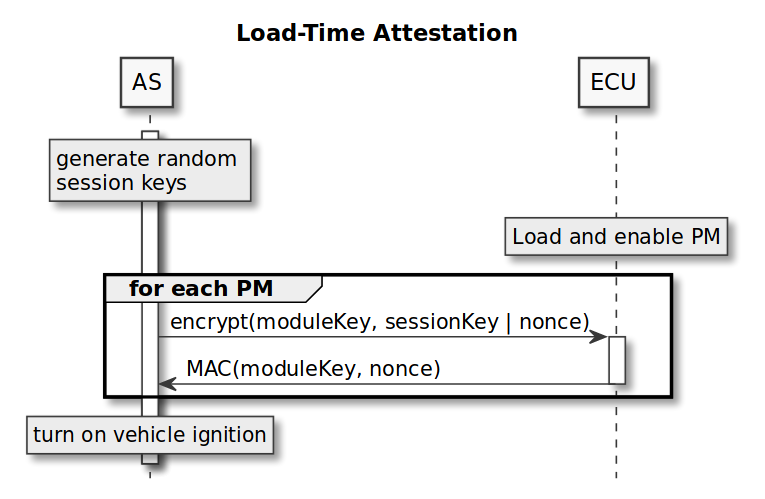
\includegraphics[width=1\linewidth]{Figures/VulCAN_attestation.png}
	\caption[]{Load-time attestation (after~\cite{VanBulck2017})}\label{fig:vulcan_load_attestation}
\end{figure}

For attesting the integrity of all loaded PMs (S3) the VulCAN protocol designed
an Attestation Server (AS) that conducts a remote attestation of all loaded PMs.
To be able to do that the AS needs the Sancus module keys for every PM\@. With
these it is easy to verify the integrity of each PM\@. A simple challenge
attestation using the module key will suffice. The challenge should contain an
nonce that monotonically increases to protect against replay attacks (P3). On
top of that, the AS can additionally provision session keys to the PMs while
attesting their integrity. This can be done by sending a random session key plus
the nonce encrypted by the respective Sancus module key to the PM\@. Only if the
PM is unmodified it can properly decrypt the session key and the nonce. Then it
can send back a valid MAC of the nonce to complete the attestation.

\begin{figure}[ht]
    \centering
    \captionsetup{justification=centering}
	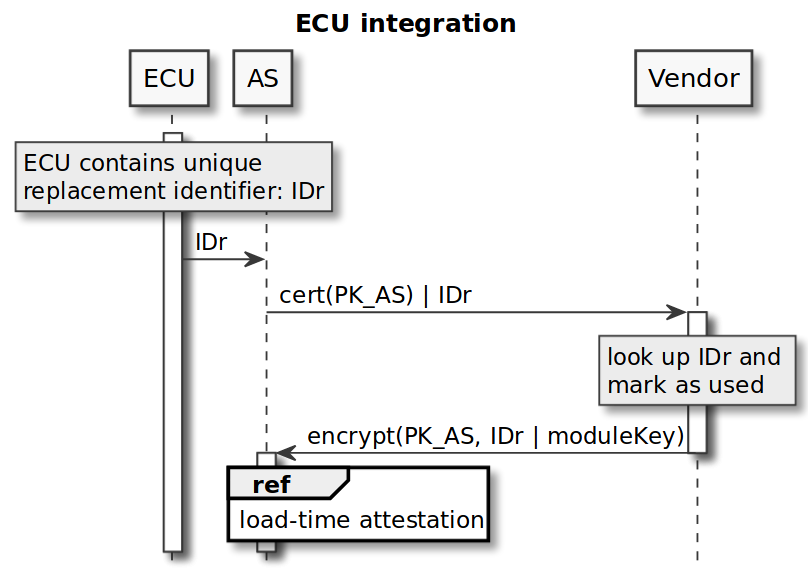
\includegraphics[width=1\linewidth]{Figures/VulCAN_ecu_replacement.png}
	\caption[]{Integration of a new ECU (after~\cite{VanBulck2017})}\label{fig:vulcan_ecu_replacement}
\end{figure}

This solves the first two challenges but leaves open how to replace an ECU by an
untrusted third party (S4). To achieve this we need to use the higher key
hierarchies from Sancus (see Chapter~\ref{subsec:sancus}). The remote car vendor
functions as the trusted infrastructure provider, it knows all root node keys of
the ECUs. It is possible to independently calculate all Sancus keys for its
ECUs. Additionally we need the AS to possess an asymmetric key. Whenever a new
component is installed into the vehicle it sends a unique replacement
identifier. The AS receives this identifier and sends it to the remote car
vendor. Together with the identifier, the AS needs to send a certificate of its
public key signed by the vendor. If the vendor positively verifies the
certificate he sends the module key of the newly installed component to the AS
encrypted with the public key of AS\@. This way only AS can decrypt the sent
module key of the new component. Subsequently, the normal attestation protocol
can be executed for the new component.

VulCAN introduces not only new software but also depends on new hardware as well
in contrast to other introduced solutions like LeiA~\cite{Radu2016} and
vatiCAN~\cite{Nurnberger2016}. However, the pure system-level security
guarantees provided by the Sancus hardware are not the only benefits gained.
With the Sancus hardware it is possible to securely shield legacy ECUs (S5). If
a security gateway is set in front of the legacy ECU to separate it from the
rest of the network, the gateway can perform all the necessary authentication as
if it were the legacy ECU\@. Due to the separate data and authentication
messages this is easily achievable. To have Gateways between CAN networks in the
vehicle network is not uncommon. But the commonly used gateways have the problem
of being insecure to exploitation or reprogramming of their
software~\cite{Checkoway2011}. If we remember, the attacker model of VulCAN
allows it to reprogram every ECU in the network which is not explicitly
protected against it. However, due to the software isolation feature of Sancus
it is possible to secure the integrity of the gateway and so properly secure the
legacy CAN network behind the gateway. The prerequisite for this to work is the
implementation of the gateway CAN driver as a Sancus PM\@. VulCANs authors think
this is acceptable because the gateway driver is considerably simplified in
contrast to a standard CAN driver.

\subsection{Security}

The VulCAN authors analyzed the security of their protocol~\cite{VanBulck2017} with the following conclusions.

\smallskip
The VulCAN protocol-level message authentication (P1) and replay attack
protection (P3) is safe against adversaries that control the network but not the
software on the ECUs. It is infeasible to brute force the session key (out of
\(2^{127}\) possibilities). Otherwise she would have to guess a correct
combination of identifier, nonce and MAC\@. Due to the non applicability of the
birthday paradox to this problem the attacker would have to guess the correct
MAC (there are \(2^{63}\) different MACs) which is also not reasonably executable
in the limited time of the session key validity. 

As a basis you ultimately have to trust the processor to be able to trust
anything running on it. And the VulCAN authors trust their Sancus~\cite{Noorman}
hardware. So their analysis regarding the system-level requirements (S2--S5) all
depend on this trusted hardware. So this leads to trust in the loaded PMs and
there communication. Through the reduction of the TCB to only these PMs and not
even trusting the system software running on the ECUs it is well within reach to
perform formal verification~\cite{Philippaerts2014} and secure
compilation~\cite{Patrignani2015}. Through the Attestation Server it is only
necessary to have once ECU with tamper-resistant persistent storage. The authors
recommend to use higher-end trusted execution technology for this like ARM
TrustZone~\cite{Alves2004} or Intel SGX~\cite{McKeen2013}. Sancus then
guarantees that only PMs with valid integrity are able to decrypt the current
session keys provided by the AS\@. The provisioning scheme of new keys by the
vendor also relies on the AS having valid integrity because when no one knows
its Secret Key no one is able to read by the vendor provided keys. Generally all
this system-level requirements depend on the trust in the execution platform at
its guarantees. The shielding of legacy ECUs depend on the protocol and
system-level guarantees that VulCAN provides. If even the CAN driver for the
gateways are executed as PMs there is no way of tampering with the gateway and
no one is able to send unauthenticated messages to the legacy components.

\subsection{Experimental Evaluation}\label{subsec:experimental_evaluation}

The VulCAN authors implemented the vulcanized versions of vatiCAN and LeiA and tested them on a testbench with six FPGA each synthesized with a Sancus-enabled OpenMSP430. These were connected with widely used MCP2515 CAN transceiver chips using a common bus with 500~kBit/s. They used the Sancus C Compiler to compile the source code.

The TCB size of the vulcanized vatiCAN version was 147 and for LeiA 212 lines of code. The total binary size of the vatiCAN / LeiA library compiled as an unprotected application was 790 / 1818 bytes. Compiled as a PM it had 906 / 1948 bytes. This does not include 22 / 44 bytes per authenticated connection that is added to the vatiCAN / LeiA binary size.

The authors made a performance evaluation and compared to the evaluation made by
the vatiCAN authors. It is to mention, that the vatiCAN authors used 16~MHz
ATmega 8-bit ECU while the MSP430 has 20~MHz and 16-bit. However, their results
should be in the same order of magnitude. The VulCAN authors found their MAC
generation (0.21ms) to be 11-times faster then the vatiCAN MAC generation
(2.95ms). The vulcanized LeiA approach with the smaller nonces took only 0.20ms.
The overall overhead for sending an authenticated message and measured
round-trip times are listed in the Appendix. In general, the VulCAN protocol with its hardware primitives for cryptography seem to make message authentication on CAN networks real-time suitable.

% !TEX root = ../report.tex

\section{Discussion}
\label{sec:discussion}

Key trade-offs \& considerations on the presented technologies for in-vehicle
communication security: VulCAN vs VatiCAN vs LeiA

maybe comparison to the internet world with tls etc. to set everything into context

% !TEX root = ../report.tex

\section{Conclusions}

This report gave a basic introduction about in-vehicle networks and then
detailed the currently published AUTOSAR-compliant message authentication
protocols. The software-only protocols LeiA and vatiCAN secure against attackers
with full access to the CAN network. However, they assume that the targeted ECUs
are not compromised. The third published message authentication protocol named
VulCAN enhances other protocols like LeiA and vatiCAN to render arbitrary code
execution on every ECU unperilous. To achieve this VulCAN uses Sancus, a trusted
execution technology with low-cost embedded devices. It enables runtime
attestation and authentication of the software components through a
hardware-only TCB\@ without breaking critical real time constraints of the
vehicle domain. Additionally VulCAN provides a way to shield legacy devices
without modifying them to help with the transition towards a secured CAN
network. 


% Can use something like this to put references on a page
% by themselves when using endfloat and the captionsoff option.
\ifCLASSOPTIONcaptionsoff
  \newpage
\fi


\bibliographystyle{abbrv}
\bibliography{bilbiography}
% that's all folks

\input{Text/Appendix}

\end{document}
